\section{Dégagement des contraintes de développement}

Selon les fonctions définies et les codes existants, j'ai défini des contraintes et proposé des solutions :


\subsection{La gestion d'utilisateurs}

\textbf{Failles} 

\begin{itemize}
    \item Manque un système d'accès connecté celui de l’écoles
    \item Sans reconnaissance d’identités
\end{itemize}

J'ai proposé :

\begin{itemize}
    \item de communiquer avec les responsables informatiques d'écoles pour intérroger les méthodes de connection
    \item de réaliser la reconnaissance selon les adresses mails \footnote{ Par exemple, @eleves.ec-nantes.fr indique un élève et @ec-nantes.fr indque un enseignant } 
    \item Avant l'intégration de comptes, un système d'autorisation provisoire ressemblant à celui d'ezb sera réalisé
    \item On pourra ajouter des messageries supplémentaires à la fin
\end{itemize}


\subsection{La gestion de livre}

\textbf{Principale Faille} est :Manque de possibilités d'utilisation de multi-format et téléchargement.

J'ai proposé :

\begin{itemize}
    \item de sauvegarder des fichiers en format XML, TEI précisement, pour son utilisation générale dans le domaine de livre numérique
    \item de chercher des outils de transformations, sinon il faut les fabriquer spécifiquement pour ezb
    \item de permettre au créateur d'un livre de définir son statut, public ou privé, pour éviter les problèmes de copyright
\end{itemize}


\subsection{La gestion de groupes}

\textbf{Faille} : Les choix concernant le créateur devraient être automatiques. 

J'ai proposé : d'ajouter des membres sans définir leur rôle individuellement.


\subsection{La gestion de projets}

\textbf{Faills}

\begin{itemize}
    \item Impossibilité de définir la finalité par utilisateur et de distribuer les parties du projet aux sous-groupes
    \item Difficulté d'organiser des citations, résumés, écritures créatives, etc dans un layer
    \item Impossibilité d'inviter d'autres éditeurs en dehors du groupe
\end{itemize}

La nouvelle conception de l'application peut être présentée dans trois parties principales, la structure de projets, la distribution de projets et la contribution aux projets.

\begin{figure}[H]
\centering
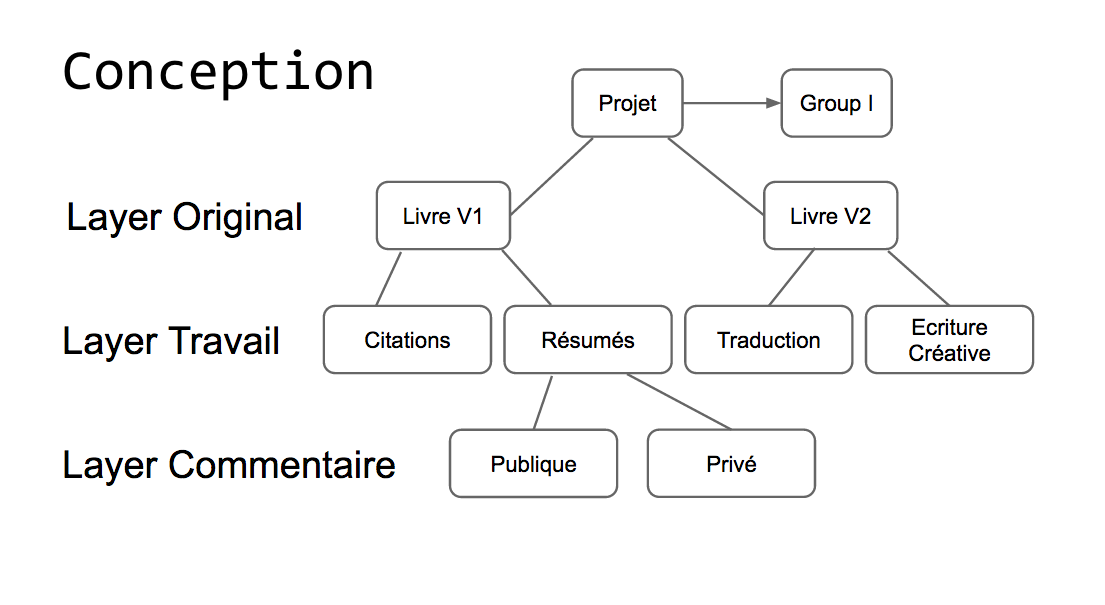
\includegraphics[width=\textwidth]{conception1}
\caption{Structure de projets}
\end{figure}

\begin{figure}[H]
\centering
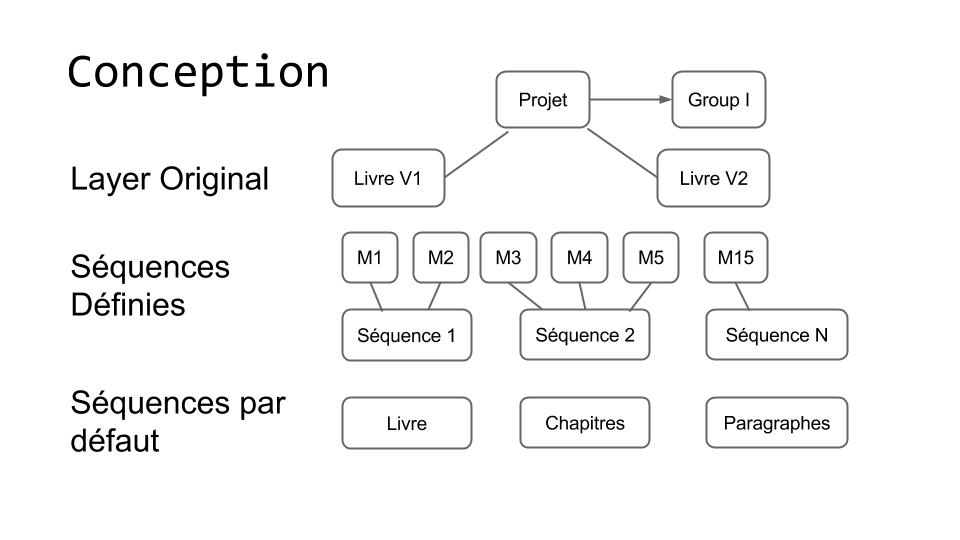
\includegraphics[width=\textwidth]{conception2}
\caption{Distribution de layers}
\end{figure}

\subsubsection{La structure de projets}

Pour garder la flexibilité du multi-échelles et la possibilité de création de layers contenant des citations et autres écritures, j'ai proposé un compromis :

\begin{itemize}
    \item Il doit être possible de choisir Privé comme le statut d'un layer qui sera ni visible pour le public ni copiable
    \item Les livres devront être traités comme layers originaux et on doit pouvoir définir des marqueurs et indiquer les séquences correspondantes
    \item On doit pouvoir créer autant de layers de travail, multi-échelles 
\end{itemize}

\subsubsection{La distribution de projets}

Les deux conceptions existantes présentent un autre problème : on ne peut pas couper un livre en plusieurs morceaux et les distribuer aux sous-groupes d'élèves selon le choix des enseignants. En même temps, il faut pouvoir proposer une segementation du livre par défaut pour simplifier de travail des managers de projets ezb. Ainsi, j'ai proposé :

\begin{itemize}
    \item d'introduire les conceptions \textbf{Marqueur}, qui indiquent une position dans le livre, et \textbf{Séquence}, qui permettent de choisir un marqueur au début, un à la fin et de distribuer ces séquences aux élèves pour un travail d'édition
    \item de permettre la distribution de séquences créées automatiquement selon une logique de livre ou chapitres ou paragraphes, etc...
\end{itemize}

\subsubsection{La contribution de projets}

\begin{itemize}
    \item Quand on veut créer un sous-layer à partir d'un layer original, on peut sélectionner l'une des séquences possibles ; les sous-layers d'un layer travail vont hériter sa segmentation automatiquement
    \item On peut avoir plusieurs choix de type d'édition quand on créé un layer :
            \begin{itemize}
                \item \textbf{Individuel} : une édition du créateur ; les membres de groupe n'ont pas le droit d'éditer
                \item \textbf{Groupe} : une édition du groupe selon la distribution des séquences du layer ; un éditeur ne peut pas voir les éditions des autres parties
                \item \textbf{Collaborative} : une édition synchronisée qui permet de lire les éditions des autres parties mais les collaborateurs du projet ne peuvent éditer que dans la partie autorisée
            \end{itemize}
    \item Les éditions d'un layer travail sont des ajouts de parties qui permettent des citations de parent-layer, des insertions et des écritures multiformat
    \item Dans les éditions d'un layer de niveau N, on peut lire tous les layers du niveau original au niveau N-1
\end{itemize}

\begin{itemize}
    \item \textbf{Layers originals} qui représentent des livres sont des bases de projets
    \item \textbf{Layers travail} garantissent une structure multi-échelles illimité et des écritures très libres
    \item D'ailleurs, la nouvelle conception de projets permet d'inviter d'autres personnes pour contribuer aux le projet ou commenter les travaux faits par des élèves. 
\end{itemize}